\documentclass[crop,tikz]{standalone}
% \usepackage[pdftex]{graphicx}
\usepackage{tikz}
\usepackage{tikz-qtree}
\usetikzlibrary{graphs,arrows.meta}
\tikzset{every tree node/.style={minimum size=2em,inner sep=1,draw,circle},
         blank/.style={draw=none},
         root/.style={draw=red,fill=red},
         proof/.style={draw=cyan,fill=cyan},
         roots/.style={draw=yellow,fill=yellow},
         edge from parent/.style={draw, edge from parent path={(\tikzparentnode) -- (\tikzchildnode)}},
         level distance=1cm}
\usetikzlibrary{calc} 
\usetikzlibrary{arrows, decorations.markings,positioning,backgrounds,shapes}
\definecolor{EMP}{HTML}{77DD77} % Green1
\definecolor{NOR}{HTML}{06500C} % Green2
\usepackage{subfig}

\begin{document}
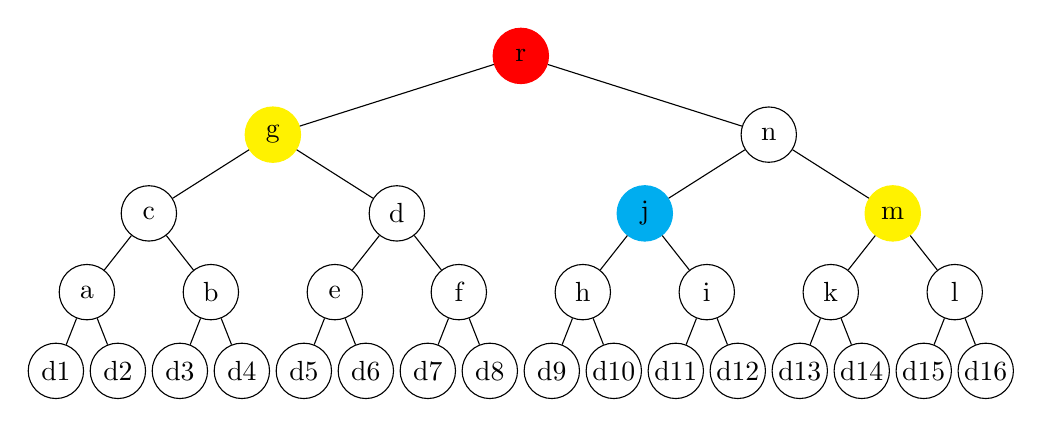
\begin{tikzpicture}
\Tree
[ .\node[root]{r};
[ .\node[roots]{g};
        [ .c   [ .a d1 d2 ]  [ .b d3 d4 ]  ]
        [ .d  [ .e d5 d6 ]  [ .f d7 d8 ]  ]
    ]
    [ .n
    [ .\node[proof]{j}; [ .h d9 d10 ] [ .i d11 d12 ] ]
        [ .\node[roots]{m}; [ .k d13 d14 ]  [ .l d15 d16 ] ]
    ] 
]
\end{tikzpicture}

% \begin{tikzpicture}
% \Tree
% [ 
% .\node[root]{r};  [ .a d1  d2 ] [ .b d3 d4 ]
% ]
% \end{tikzpicture}

\end{document}
